\chapter{Progettazione e codifica}
\label{cap:progettazione-codifica}

%Mettere i mockup di figma con spiegazione
%riportare una analisi del codice e la fatica fatta con firebase


\intro{Breve introduzione al capitolo}\\

\section{Progettazione}
\label{sec:progettazione}
%partire dicendo di aver progettato l'interfaccia con figma, riportando degli screen dal mio lavoro

\subsection{Struttura dell'app}

Dopo una prima parte di stage dove ho studiato le tecnologie riportare al \hyperref[sec:tecnologie]{terzo capitolo}, ho pensato come sviluppare l'applicazione richiesta.\newline
Di prassi in RiskAPP si utilizza Figma per poter avere una idea più chiara del lavoro che si desidera fare, quindi per prima cosa ho progettato la grafica e la struttura dell'app con l'aiuto di questo software di progettazione.\newline
Avendo una idea visiva, questo rendeva più facile spiegare al mio tutor come pensavo di impostare l'applicazione, andando poi a modificare e sistemare in base alle esigenze dell'azienda.\newline
\newline
Nella figura \ref{fig:schermatefigma} ci sono tre schermate progettate in Figma, ovvero le schermate \textbf{Utente}, \textbf{Impostazioni} e infine \textbf{Home}.\newline
Dai \emph{mockapp} capiamo che la struttura delle pagine è la seguente:
\begin{itemize}
    \item una barra superiore, dove è possibile eseguire un paio di azioni;
    \item una schermata con le informazioni interessate;
    \item una barra di navigazione, fatta eccezzione per la schermata \textbf{Impostazioni} che non è presente.
\end{itemize}
Nella barra di navigazione è possibile andare alle schermate:
\begin{itemize}
    \item \textbf{Home} dove sarà visibile la \emph{\gls{cassacomuneg}}, la \emph{\gls{quotastornatag}} dell'utente e infine il piatto del giorno (successivamente cambiato in \emph{Proposte del giorno} per permettere la scelta di più piatti dal menu);
    \item \textbf{Spese} che permette di visualizzare tutte le transazioni di tutti gli utenti e aggiungere delle nuove transazioni o eliminarle;
    \item \textbf{Menu} dove è possibile consultare i piatti, aggiungerli oppure proporli come possibili piatti del giorno;
    \item \textbf{Utente} la visualizzazione cambia tra utente semplice e utente amministratore ed è stata modificata durante la fase di codifica, ma rincipalmente serve per visualizzare e modificare le proprie presenze o, nel caso dell'amministratore, modificare le presenze degli stagisti e la \emph{\gls{quotapastog}}.
\end{itemize}
\begin{figure}[!h]
    \centering 
    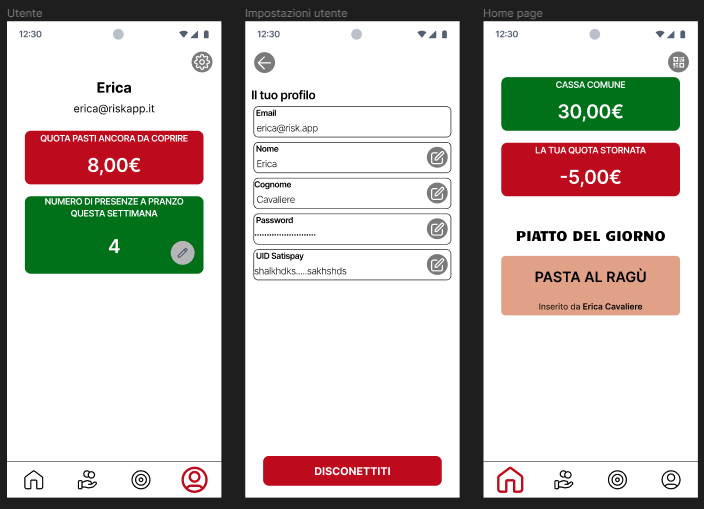
\includegraphics[width=1.0\columnwidth]{figma/esempi} 
    \caption{Alcune schermate progettate in Figma}
    \label{fig:schermatefigma}
\end{figure}
La schermata \textbf{Impostazioni} è raggiungibile attraverso la schermata \textbf{Utente}, andando a toccare l'icona ad ingranaggio posta nella barra superiore.\newline
Da \textbf{Impostazioni} è possibile modificare i dati dell'utente oppure permettere all'utente di disconnettersi dalla sessione corrente.\newline
\newline
Sono state create diversamente anche le finestre Accedi (Figura \ref{fig:accedifigma}) e Registrati (Figura \ref{fig:registratifigma}).\newline
In queste due schermate non sono presenti barre superiori o inferiori, ma solo una serie di campi da compilare e il pulsante verde Accedi o Registrati.\newline
La schermata Accedi deve essere la prima schermata che vede l'utente quando entra nell'app e per passare alla schermata Registrati, bisogna andare a toccare il link presente sotto al pulsante Accedi, dove è presente il messaggio "Sei nuovo? REGISTRATI"
Per ritornare alla schermata Accedi, il procedimento è analodo, ovvero si tocca il link presente sotto il pulsante, dove viene riportato il messaggio "Hai già un account? ACCEDI".\newline
Invece, per andare nella schermata Home, bisognerà compilare correttamente i campi e poi toccare il pulsante presente nella schermata.\newline
\newline
Nella schermata Accedi è presente anche il messaggio "Hai dimenticato la password?", questo doveva contenere un link che permetteva all'utente di recuperare e modificare la password, ma poi questo messaggio è stato tolto in accordo con il mio tutor, perchè per l'uso dell'app il recupero password non aveva alcuna utilità.\newline
\begin{figure}[!h] 
    \centering 
    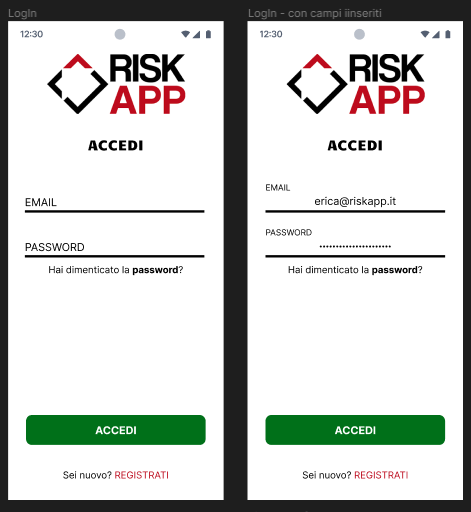
\includegraphics[width=0.7\columnwidth]{figma/accedi} 
    \caption{Schermata Accedi progettata in Figma}
    \label{fig:accedifigma}
\end{figure}
\begin{figure}[!h] 
    \centering 
    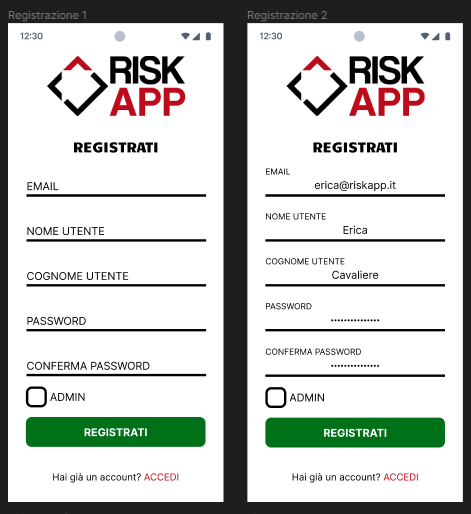
\includegraphics[width=0.7\columnwidth]{figma/registrati} 
    \caption{Schermata Registrati progettata in Figma}
    \label{fig:registratifigma}
\end{figure}

\newpage

\begin{figure}[!h] 
    \centering 
    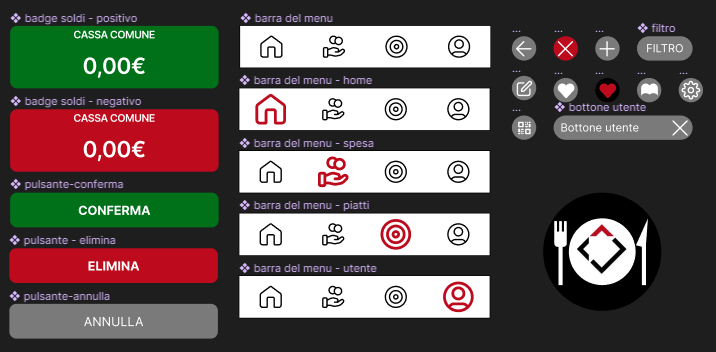
\includegraphics[width=0.9\columnwidth]{figma/container} 
    \caption{Alcuni pulsati e icone progettate in Figma}
    \label{fig:conteinerfigma}
\end{figure}

\newpage

\subsection{Database}

\begin{figure}[!h] 
    \centering 
    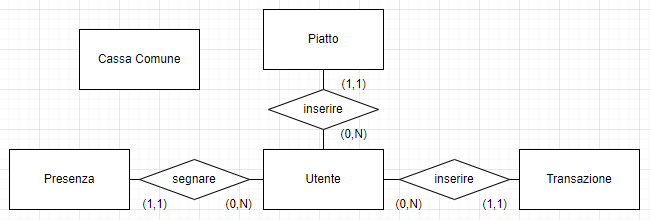
\includegraphics[width=0.9\columnwidth]{database} 
    \caption{Il database progettato per l'applicazione}
    \label{fig:database}
\end{figure}

\newpage

\section{Design Pattern utilizzati}
%forse parlare dell'MVVM o BLoC patttern

\section{Codifica} %riportare qui il database?
%In questa sezione riporto la struttura della cartella lib, parlerò delle componenti e, del file firebase_option e delle classi
%riportare anche le immagine dell'app creata